%!TEX program=xelatex
\documentclass{article}
\usepackage{ctex}

% Set page size and margins
% Replace `letterpaper' with `a4paper' for UK/EU standard size
\usepackage[letterpaper,top=2cm,bottom=2cm,left=2.5cm,right=2.5cm,marginparwidth=1.75cm]{geometry}

% Useful packages
\usepackage{amsmath}
\usepackage{graphicx}
\usepackage{float}
\usepackage[colorlinks=true, allcolors=blue]{hyperref}

\title{微分方程数值解计算实习课后作业2}
\author{陈文宇}
\date{\today}


\begin{document}


\maketitle

\tableofcontents

\newpage
%---------------------------------------------------
\section{问题重述}
测试不同基函数对求解的影响:例$1.4.1$
\[
\left\{
\begin{aligned}
	&\mu '' + \mu = -x &0<x<1 
	\\
	&\mu(0)=\mu(1)=0 &
\end{aligned}
\right.
\]

取基函数为
$$\phi_{i}(x)=\sin(i\pi x) 以及 \phi_{i}(x)=(1-x)x^{i},i=1,2,\dots,N.$$

\begin{itemize}
    \item 对比两组基函数对应的系数矩阵的条件数随着N增加产生的变化
    \item 画图对比两组基函数对应的数值解和精确解$$\mu_{*}(x)=\frac{\sin{x}}{\sin{1}}-x$$
    之间的 $L^{2}\{[0,1]\}$误差:
    $$ err=(\int^{1}_{0}(\mu_{*}(x)-\mu_{n}(x))^{2})^{\frac{1}{2}}$$
    随着N增加产生的变化
\end{itemize}
 
%---------------------------------------------------
\section{实验思路}
使用Ritz-Galerkin方法,只需求解线性方程组$Ax=b$,
对于条件数可以使用matlab命令$cond(A,2)$,
err的求解可以使用复化Simpson方法来求解,
进而使用plot函数绘制图像即可。

具体的操作:
\begin{itemize}
    \item 将$A(i,j)$公式写成函数Aijeqution.m计算系数矩阵,使用命令$cond(A,2)$计算条件数
    \item 将$b(i)$公式写成函数bieqution.m计算右端向量,使用$x=A\backslash b'$ 求解线性方程,即可获取微分方程数值解
    \item 使用复化Simpson方法来求解误差$err$,并绘图,这些操作保存在 main.m 中
      
\end{itemize}


%---------------------------------------------------

\section{实验结果}
下列表格是对基函数个数$N$与系数矩阵条件数$condA$

\begin{table}[h]
  \centering
    \begin{tabular}{|c|c|c|c|c|c|c|c|c|c|c|}
    \hline
    N     & 1     & 2     & 3     & 4     & 5     & 6     & 7     & 8     & 9     & 10 \\
    \hline
    $conA$ & 1     & 4.34  & 9.9   & 17.69 & 27.71 & 39.95 & 54.41 & 71.1  & 90.02 & 111.16 \\
    \hline
    N     & 11    & 12    & 13    & 14    & 15    & 16    & 17    & 18    & 19    & 20 \\
    \hline
    $conA$ & 134.53 & 160.12 & 187.94 & 217.99 & 250.25 & 284.75 & 321.47 & 360.42 & 401.59 & 444.99 \\
    \hline
    \end{tabular}
    \caption{\label{三角多项式基底下的条件数变化}三角多项式基底下的条件数变化}
\end{table}

\begin{table}[h]
  \centering
  \scalebox{0.9}{
    \begin{tabular}{|c|c|c|c|c|c|c|c|c|c|c|}
    \hline
    N & 1 & 2 & 3 & 4 & 5 & 6 & 7 & 8  & 9  & 10 \\
    \hline
    $conA$ & 1 & 10.17 & 161.10 & 3106.29 &6.69E+04& 1.55E+06 & 3.80E+07 & 9.66E+08 & 2.53E+10 & 6.8E+11 \\
    \hline
    \end{tabular}
    }
  \caption{\label{代数多项式基底下的条件数变化}代数多项式基底下的条件数变化}
  
\end{table}

\newpage
下列图像是基函数个数$N$与误差$err$的图像:
\begin{figure}[H]
\centering
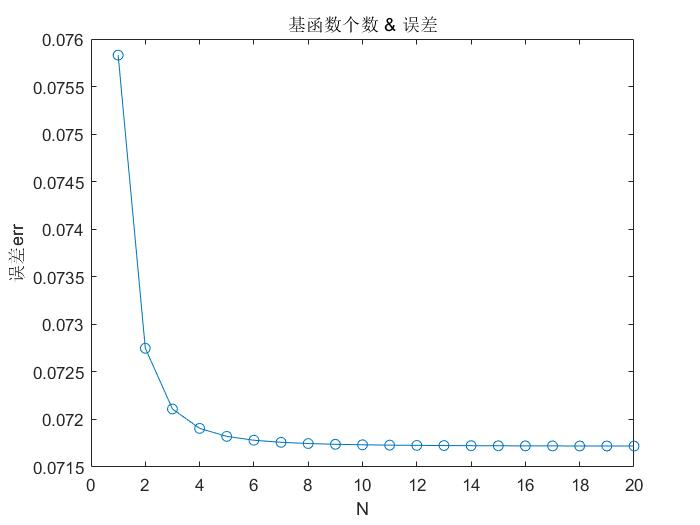
\includegraphics[scale=0.4]{N_err_1.jpg}
\caption{\label{N_err_1}三角多项式作为基函数}
\end{figure}

\begin{figure}[H]
\centering
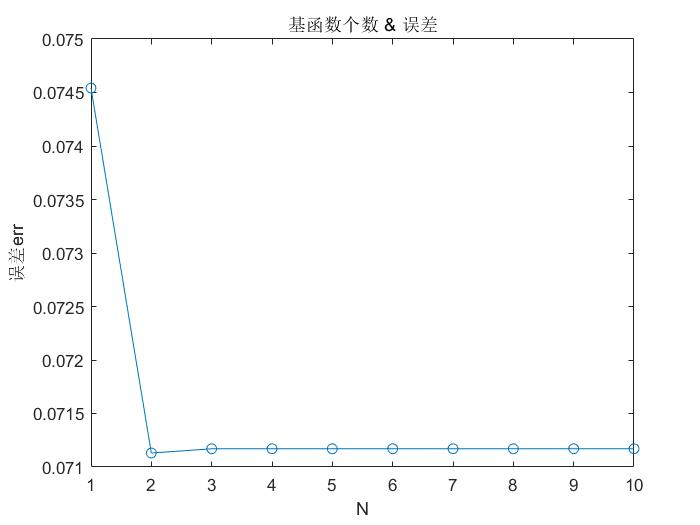
\includegraphics[scale=0.4]{N_err_2.jpg}
\caption{\label{N_err_2}代数多项式作为基函数}
\end{figure}



\newpage
%-----------------------------------------------------
\section{实验结果分析}
随着基函数个数的增加,两类基底下系数矩阵的条件数都在逐渐增大。

对于三角多项式基底,我绘制了N与$\sqrt{\|A\|}$的图像,可以看出$\|A\|=O(N^{2})$。这是简单的,因为对角矩阵的条件数是最大奇异值和最小奇异值的比值,即$$condA=\frac{(N\pi)^{2}-1}{\pi^{2}-1}$$
\begin{figure}[H]
\centering
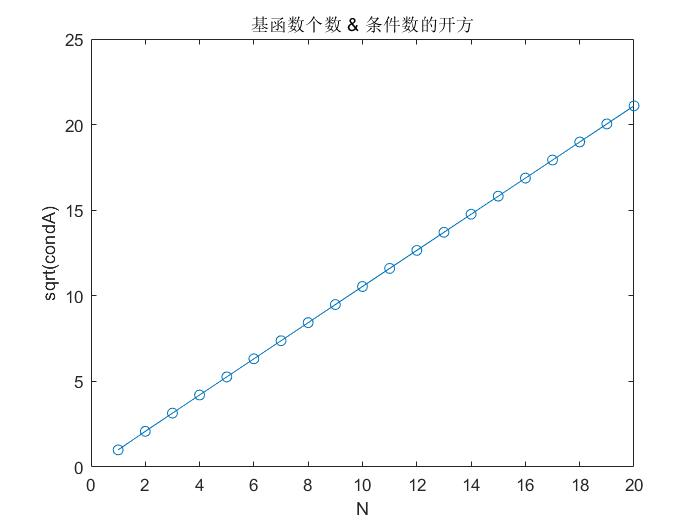
\includegraphics[scale=0.39]{N_sqrt_condA.jpg}
\caption{\label{N_sqrt_condA}三角多项式基底下,N与$\sqrt\|A\|$的图像关系图}
\end{figure}
对于代数多项式基底,我绘制了N与$\log{\|A\|}$ 的图像,可以看出$\|A\|=O(e^{N})$,并且当$N>12$,系数矩阵的条件数过大,matlab报告“警告:矩阵接近奇异值,或者缩放错误。结果可能不准确”.
\begin{figure}[H]
\centering
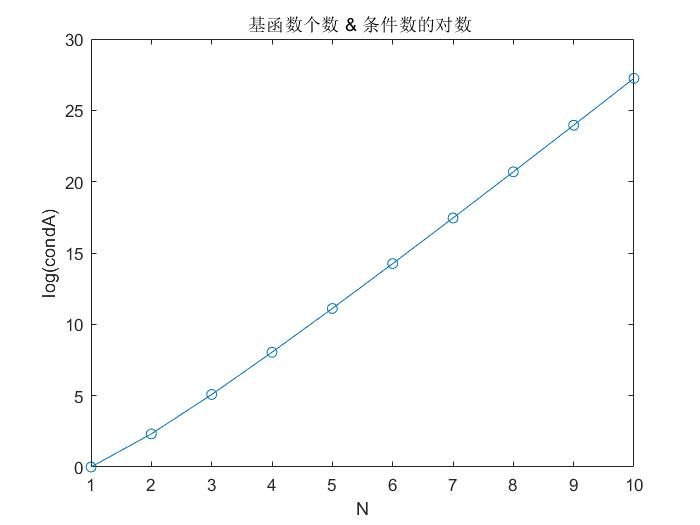
\includegraphics[scale=0.39]{N_logcondA.jpg}
\caption{\label{N_logcondA}代数多项式基底下,N与$\exp{\|A\|_{2}}$的图像关系图}
\end{figure}

随着基函数个数的增加,两类基底下误差都在逐渐减小。

\end{document}